\raggedbottom
\section{Set Construction and Filtering}
\label{app:benchmarks}

\subsection{Passages, concepts and future questions}

The primary generator is GPT-4.1. Each episode contains a passage,
candidate concepts with gold utility labels, and a future question and
answer. Explicit places the useful concept in the passage.
\textbf{Implied-answer} training episodes cue an unstated useful concept
that supplies the answer, including episodes from the
alternate-generator set.  Decoupled requires an unstated bridge to support a
further inference: the answer is absent from the passage and candidate
set, and the question shares no passage content word except a
protagonist's name. Compositional requires a multi-hop inference and
permits question anchors from the passage. Decoupled and Compositional
are development sets used for configuration selection and excluded from
gradient training.

Rule-based validation checks candidate strings, bridge absence, answer
exclusion and the Decoupled question's lexical overlap. Concept
deduplication removes repeated concepts across retained episodes, while
leakage filtering also checks full lexemes, inflected answers and
question anchors. A blind GPT-6-Astra alias filter receives the future
question, gold answer and bridge. It rejects identity, morphological or
derivational variants, synonyms, translations, abbreviations and
containment that trivially yields the answer. For example,
\emph{caterer/catering} is an alias, whereas \emph{Madrid/Spanish}
requires a further inference.

\subsection{Episode-generation prompt}
\label{app:authorprompt}
GPT-4.1 receives the system instruction, ``You are a careful dataset
designer for a cognitive-science experiment on LLM memory.'' The
following prose transcription preserves the generation constraints
(Prompt~\ref{prompt:author}); the output-format instruction requests one
structured record per episode. Generation uses temperature 1.0 and
batches of up to five episodes, after which rule-based filters and the
alias filter apply.

\subsection{Held-out and replication sets}
\label{app:fresh}

The held-out set and test set use the Decoupled
construction prompt and rule-based filters, followed by deduplication
and disjointness filtering. A context match after lowercasing and
trimming against a prior set causes exclusion. A bridge that matches a
labeled useful concept of the training episodes also causes exclusion.
The test set also excludes contexts appearing in the held-out set. Shared answer categories, such as languages and
currencies, are permitted. The retained sets contain 316 and 363
episodes, respectively. The alternate-generator set repeats the
Implied-answer construction with GPT-4o, and the entity-bridge set comes from GPT-5.6 (App.~\ref{app:replications}).
Training and validation splits contain 175 and 45 episodes,
respectively, from 88 Explicit episodes and 132 episodes in which the
passage cues an unstated useful concept that supplies the answer,
including the 57-episode alternate-generator set.

Development uses Decoupled (68 episodes), Compositional (52), and two
separate 68-episode sets adding confusable or unrelated unstated
distractors to Decoupled. The held-out set and the test set contain
316 and 363 episodes, respectively, while the entity-bridge set
contains 42 episodes.

\subsection{Reconstructing the reported controls}
\label{app:pools}
\label{app:controls}

All pool interventions traverse the 363 test-set episodes in
their fixed order and preserve the question, answer and original
utility labels. Added candidates receive negative utility labels.
Within an episode, original candidates precede additions, which keep a
fixed order. The original pool contains 1,607 candidates,
4.43 per episode. Statedness uses the case-insensitive stem match
specified in \S\ref{sec:setup}. Table~\ref{tab:pools} summarizes every pool and control, including its construction, candidates per episode and what it isolates.

\paragraph{Worked source episodes.}
Figure~\ref{fig:examples} gives the first two test-set episodes
in full; the second is the episode drawn in Figure~\ref{fig:episode}.

\begin{figure*}[t]
\centering
\begin{minipage}[t]{0.485\textwidth}
\begin{sdabox}[example]{First test-set episode}[ex:yara]
\textbf{Passage.} Yara compared renewal quotes from different insurers
online and reviewed her accident history. She called the hotline to ask
clarifying questions about premium increases. After considering the
coverage limits and deductibles, Yara finally entered her payment
details to confirm the policy.

\medskip
\textbf{Candidates, in supplied order.} insurer, deductible, history,
policy, insurance.\\
\textbf{Useful concept.} insurance. \textbf{Surface distractors.}
deductible, history. \textbf{Neutral concepts.} insurer, policy.

\medskip
\textbf{Future question.} Which professional would be most relevant for
Yara to contact regarding her recent purchase?\\
\textbf{Answer.} agent.
\end{sdabox}
\end{minipage}\hfill
\begin{minipage}[t]{0.485\textwidth}
\begin{sdabox}[example]{Second test-set episode}[ex:jibril]
\textbf{Passage.} Jibril had always wanted to gaze up at the world's
highest outdoor observation deck. Early one morning, he took a swift
elevator to level 148 of the Burj Khalifa, joining a crowd of eager
tourists. Below him, the city sparkled with the first rays of the desert
sun. After snapping several panoramic photos, he browsed the sleek gift
shop for souvenirs.

\medskip
\textbf{Candidates, in supplied order.} elevator, desert, gift,
observation, dubai, tourists.\\
\textbf{Useful concept.} dubai. \textbf{Surface distractors.} desert,
tourists. \textbf{Neutral concepts.} elevator, gift, observation.

\medskip
\textbf{Future question.} What language was Jibril most likely to hear
from local staff during his visit?\\
\textbf{Answer.} arabic.
\end{sdabox}
\end{minipage}
\caption{First two test-set episodes in full. Admission sees only
the passage and candidate strings; utility labels, questions and answers
are included for explanation.}
\label{fig:examples}
\end{figure*}


\begin{table*}[t]
\centering
\caption{Candidate pools and controls, their construction, candidate counts, and the comparisons they support.}
\label{tab:pools}
\small
\begin{tabular}{*{4}{p{\dimexpr\textwidth/4-2\tabcolsep\relax}}}
\toprule
Pool or control & Construction & Candidates per episode & What it isolates \\
\midrule
Original pool & Original passage and candidates & 4.43 & Reference composition \\
Statedness-balanced pool & State useful concept at even positions; add unstated candidates & 7.93 & Useful-concept statedness \\
Naming-balanced pool & Name four candidates at varied positions & 7.93 & Candidate naming and sentence position \\
Pool with unstated distractors & Append accepted same-topic distractors & 8.42 & Ranking among unstated candidates \\
Enlarged pool & Add same-topic and cross-episode distractors & 12.41 & Candidate-pool size \\
Stated-bridge control & Append sentence naming useful concept & as original & Useful-concept statedness \\
Position control & Prepend sentence naming useful concept & as original & Naming-sentence position \\
Distractor-named control & Append sentence naming first non-useful candidate & as original & Distractor naming \\
Passage replacement & Permute passages; retain candidates and labels & as original & Passage dependence \\
Useful-concept replacement & Substitute next-ranked candidate for selected useful concept & as original & Effect of useful-concept retention \\
Paired-passage set & Paired passages; App.~\ref{app:pairedpassage} & 8.86 & Paired-passage comparison \\
\bottomrule
\end{tabular}
\end{table*}

\paragraph{Construction rules.}
The stated-bridge control appends ``The passage also mentions \emph{concept}.'' with the useful concept substituted. The position control prepends this sentence. The distractor-named control appends it with the first non-useful candidate in the original order.

For the pool with unstated distractors, an LLM is asked for four lowercase single-word concepts from the useful concept's semantic category: alternatives a careless reader might confuse with it, absent from the passage and not implied by it. The response must be comma-separated. Response order is retained. A concept matching an original candidate or occurring as a case-insensitive substring of the passage is discarded; accepted concepts are appended. This gives 1,450 additions: four in 361 episodes and three in episodes 24 and 263, for 3,057 candidates. The development confusable-distractor control applies this procedure to Decoupled.

For the statedness-balanced pool, odd positions, counting from one, retain the original passage; even positions append the naming sentence with the useful concept. Every episode retains its original candidates and appends the first four accepted additions at odd positions or the first three at even positions from the pool with unstated distractors, preserving order. This gives 2,877 candidates.

The naming-balanced pool uses the same ordered candidate lists and starts from the original passages. It names four candidates per episode: four other candidates at odd positions, or the useful concept and three others at even positions. One generator seeded with zero samples uniformly without replacement in fixed episode order. Selected candidates are shuffled before naming sentences are constructed. The five sentence forms rotate: ``The passage also mentions \emph{concept}.'', ``\emph{concept} is relevant here.'', ``Note that \emph{concept} comes up as well.'', ``There is also \emph{concept} to consider.'', and ``\emph{concept} features in this as well.'' The first selected candidate uses the form at the episode's position in this cycle; subsequent candidates advance one form. Insertion boundaries vary with episode and insertion index, using the current sentence list including earlier additions. There are 1,452 naming sentences, 181 naming the useful concept.

The enlarged pool concatenates the original candidate list, accepted same-topic additions, and four useful concepts from subsequent episodes, in that order. Selection starts with the next episode and advances cyclically, accepting a useful concept only when it is absent from the passage and original list and distinct from earlier accepted cross-episode concepts. Selection stops after four accepted concepts. Concatenation retains the first occurrence of each concept, giving 4,506 candidates. The development unrelated-distractor control uses only the original candidates and these four cross-episode additions.

In the original pool, the useful concept is stated in 5\% of test-set episodes and negative candidates in 99\%. In 95\% of episodes, the useful concept is the sole unstated candidate.

\paragraph{Passage and useful-concept replacement.}
Passage replacement uses a fixed episode permutation to replace each passage while preserving its candidates, utility labels, question and answer. Useful-concept replacement acts on SDA's top-two selections only when they contain the useful concept. It retains the other selection and substitutes the next-ranked candidate for the useful concept; the same frozen reader then answers the same question again. This yields 249 replacement episodes (App.~\ref{app:episodemetrics}).

\paragraph{Paired-passage set.}
\label{app:pairedpassage}
We construct the paired-passage set from the 363 test-set episodes. Matching these episodes into 181 disjoint pairs
yields 362 episodes, with each source episode in at most one pair and
one episode unpaired. Each member retains its passage, future question,
and answer. Its own useful concept is the only candidate with a
positive gold label, and its partner's useful concept is a negative
candidate. Each member's candidate list is the union of the two
original lists, averaging 8.86 candidates per episode, with between
8 and 12 candidates. Pair members contain the same candidates in
different shuffled orders; no member retains its source order.
In all 362 episodes, no useful concept appears as a word in either
passage of its pair. Word presence therefore cannot separate the
useful concept from the partner's useful concept; only the content of
the passage can. SDA's configuration was fixed before this set was
built.
Figure~\ref{fig:pairexample} shows one complete pair.

\begin{figure*}[t]
\centering
\begin{minipage}[t]{0.485\textwidth}
\begin{sdabox}[example]{Paired-passage set, first episode}[ex:pairA]
\textbf{Passage.} Soraya carefully arranged the menorah on the windowsill, lighting the first candle at sunset. Her family gathered, singing traditional songs and spinning dreidels. Plates of latkes and sufganiyot were passed around. The evening was filled with laughter and storytelling, each tale passed down for generations.

\medskip
\textbf{Candidates, in supplied order.} clients, bouquets, lilies, florist, hanukkah, song, latke, candle, holiday, vases.\\
\textbf{Useful concept.} hanukkah.

\medskip
\textbf{Future question.} What religion does Soraya traditionally observe during this holiday?\\
\textbf{Answer.} judaism.
\end{sdabox}
\end{minipage}\hfill
\begin{minipage}[t]{0.485\textwidth}
\begin{sdabox}[example]{Paired-passage set, second episode}[ex:pairB]
\textbf{Passage.} Minh spent the afternoon arranging yellow and white lilies in tall crystal vases. She snipped stems and removed wilted leaves to ensure the displays would last. After consulting her chart, she delivered the finished bouquets to waiting clients preparing for a special event downtown.

\medskip
\textbf{Candidates, in supplied order.} florist, latke, song, holiday, clients, vases, candle, bouquets, hanukkah, lilies.\\
\textbf{Useful concept.} florist.

\medskip
\textbf{Future question.} What might Minh worry about if her workplace got too cold overnight?\\
\textbf{Answer.} freezing.
\end{sdabox}
\end{minipage}
\caption{One pair from the paired-passage set. Both passages leave
\emph{hanukkah} and \emph{florist} unstated and share ten candidates in
different orders; the passage determines which candidate is useful.}
\label{fig:pairexample}
\end{figure*}

\FloatBarrier
\section{SDA Training and Scoring Details}
\label{app:training}

\subsection{Teacher construction and data split}

Within each episode, let $r_S(c)$ be a candidate's ascending mid-rank
under score $S$, with ties assigned the average of their occupied
ranks. For $m>1$ candidates, the percentile is
\begin{equation}
P_S(c;x)=\frac{r_S(c)-1}{m-1},
\qquad S\in\{W,\mathrm{LL}\}.
\label{eq:percentile}
\end{equation}
For a singleton pool the percentile is one half. Averaging the
percentiles yields the teacher in Eq.~\eqref{eq:teacher}; descending
teacher score and then candidate order determine the top-2 labels.

A source group is one generator-and-construction group: Explicit
(88 episodes), implied-answer from the primary generator (75), or
implied-answer from the alternate generator (57). The split is
stratified by these groups and assigns whole episodes, including all
their candidates, to training or validation. Within each group,
episodes are sorted by a hash of the source-qualified episode identity
under a fixed seed; the lowest 20\%, rounded up, enter validation. The
three groups respectively contain 70 training
and 18 validation episodes, 60 training and 15 validation episodes,
and 45 training and 12 validation episodes, giving 175 training and
45 validation episodes in total. The selection protocol is specified
in \S\ref{sec:student}.

\subsection{Complete training configuration}
\label{app:configuration}

\begin{figure*}[t]
\centering
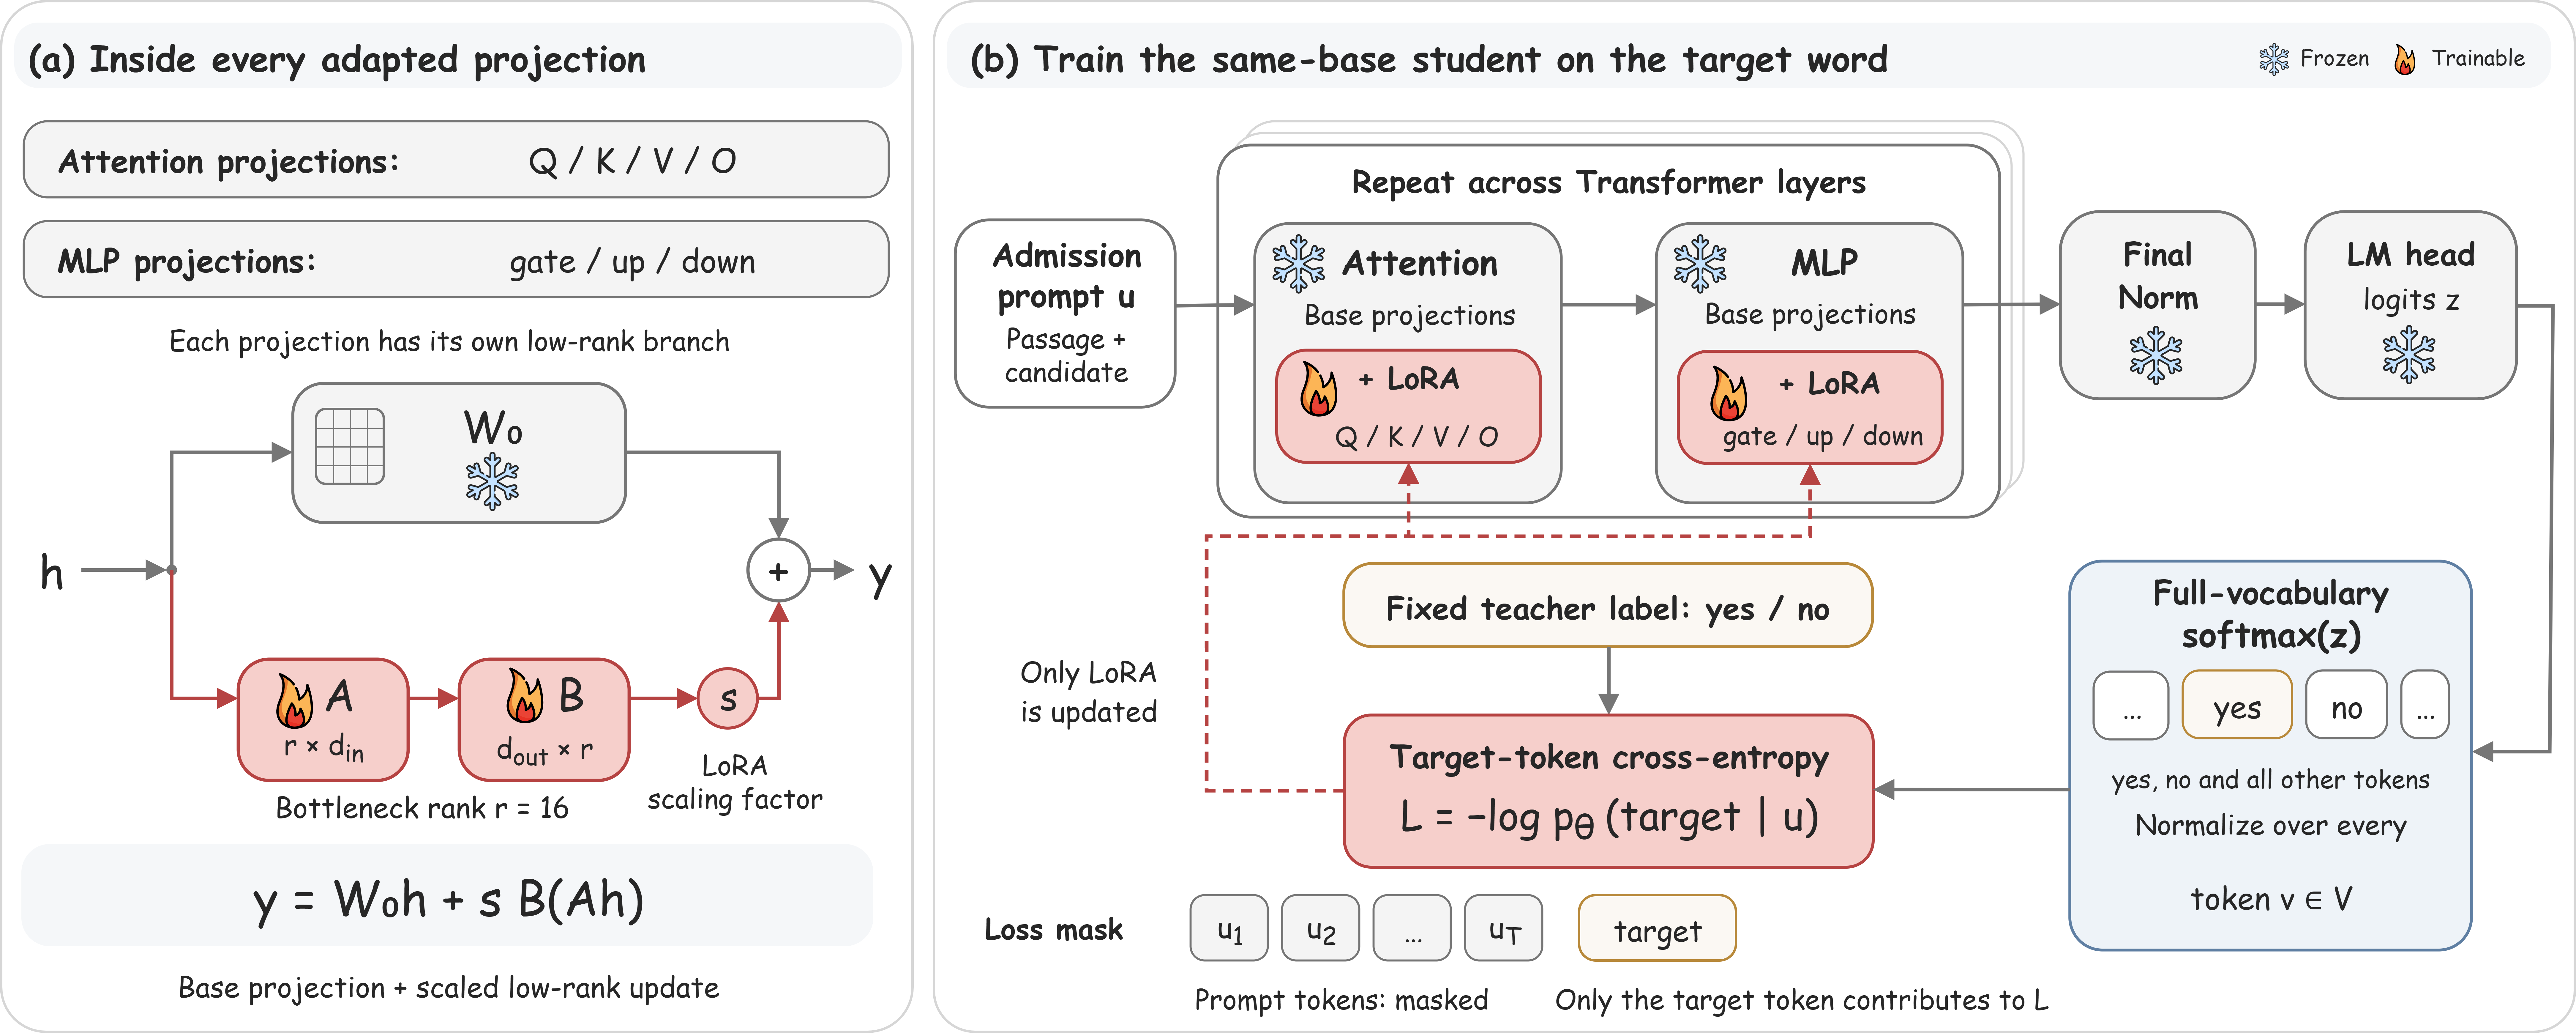
\includegraphics[width=\textwidth]{figures/fig4.png}
\caption{SDA trains an adapter while keeping base parameters frozen. (a) LoRA updates modify attention and feed-forward projections. (b) Only the teacher's target word contributes to vocabulary-normalized cross-entropy.}
\label{fig:appadapter}
\end{figure*}

LoRA adapts the attention query, key, value and output projections and
the feed-forward gate, up and down projections
(Figure~\ref{fig:appadapter}). Base parameters remain frozen. Only the
target word contributes to the vocabulary-normalized
cross-entropy in Eq.~\eqref{eq:loss}. Prompt tokens are masked. Qwen3 uses its chat template with thinking disabled. The short names Qwen2.5-7B, OLMo-2-7B and Mistral-7B denote the instruct checkpoints Qwen2.5-7B-Instruct, OLMo-2-1124-7B-Instruct and Mistral-7B-Instruct-v0.3.

\begin{center}
\small
\begin{tabular}{@{}p{0.30\linewidth}p{0.64\linewidth}@{}}
\toprule
Setting & Configuration \\
\midrule
Adapter & Low-rank adaptation, rank 16, scaling 32; attention and
feed-forward projections \\
Optimizer & AdamW; constant learning rate $1\times10^{-5}$ \\
Batching & Batch size 1; gradient accumulation over 4 batches \\
Training duration & Two epochs; 414 optimizer steps \\
Sequence length & At most 1024 tokens \\
Data & 175 training and 45 validation episodes; source-stratified, disjoint episodes \\
Targets & Two highest teacher ranks positive; all others negative \\
\bottomrule
\end{tabular}
\end{center}

\subsection{Admission baselines}
\label{app:baselines}

SDA is compared with the following baselines. The \textbf{importance
report} uses the untrained model's score $V$ in Eq.~\eqref{eq:score}.
The \textbf{1--10 importance rating} is the expected rating under
normalized probabilities of the complete answer strings.
The \textbf{reversed importance report} admits the lowest-scoring
candidates. \textbf{Unstated-first} prioritizes candidates absent from
the passage under the statedness test and breaks ties at random.
\textbf{Unstated-first with report ordering} prioritizes unstated
candidates and uses the importance report to order candidates within
each statedness class. The \textbf{statedness-adjusted report} adds a
single coefficient times the candidate's statedness indicator to the
untrained report, with the coefficient fitted on development episodes
and held fixed for evaluation. The \textbf{combined teacher used
directly} ranks by Eq.~\eqref{eq:teacher} without training an adapter.
The \textbf{implied-content wording} permits implied content; the
\textbf{statedness-cued wording} explicitly says the passage may never
mention the useful concept (App.~\ref{app:wording}).
\textbf{Random selection} samples candidates uniformly; \textbf{output
likelihood} and the \textbf{workspace readout} rank candidates directly
by their respective scores. \textbf{Gold-concept selection} ranks the
labeled useful concept first; the closed-book and full-context readers
provide accuracy references.

A single statedness offset for stated candidates, fitted on development
episodes, places every unstated candidate ahead of every stated
candidate, turning the report into unstated-first with report ordering.
It raises development AUC from 0.304 to 0.978 while lowering
statedness-balanced AUC from 0.683 to 0.575. Accuracy matches this
rule at $k=2,3$; at $k=1$, the offset and rule reach 36.6\% and 36.9\%,
respectively. Unlike this offset, SDA's ranking depends on the passage
(\S\ref{sec:ablations}, Figure~\ref{fig:mechanism}c).

\subsection{Published admission criteria as implemented}
\label{app:publishedbaselines}

\paragraph{ConsistencyGate.}
ConsistencyGate \citep{consistencygate2026} is a write-time gate that
scores how strongly the source context supports a candidate fact. We
measure two forms. The sampled form follows their Equations~2 and~3,
using their Appendix~C prompt verbatim with five samples at temperature
one and at most eight new tokens per sample. Its score is the mean of
the parsed decimals. The single-pass form follows their Equation~4
variant: the same question is posed as a yes/no question, and the score
is the probability of yes from a softmax over the yes and no token
log-probabilities. Ranking uses the score itself under the shared
top-$k$ budget, and their 0.7 threshold enters only the gate-rate diagnostic. On the original pool, ConsistencyGate's 0.7 threshold admits 26.7\% of useful concepts against 70.8\% of all candidates. Its within-episode AUC is 0.133 for single-pass scoring and 0.190 for sampled scoring.

\paragraph{A-MAC.}
A-MAC \citep{amac2026} is a multi-factor value model. Utility is obtained
from one temperature-zero call asking whether the candidate is
actionable, supports likely follow-up questions, or captures a
persistent constraint or preference. Confidence is the maximum ROUGE-L
between the candidate and a supporting passage sentence. The type prior
is their rule-based entity cue. Their novelty term compares against
memory already held, and their recency term decays with elapsed time.
Within an episode, memory is empty at the first admission and all
candidates share one timestamp, so neither term orders candidates.
These two terms are therefore omitted from the ranking score. The
three remaining factors are combined as a weighted sum, with the
utility weight fixed at one. Confidence and type-prior weights are
searched on a grid from 0.0 to 2.0 in steps of 0.1, selected by
within-episode AUC inside five-fold cross-validation over the 363
episodes, and evaluated out of fold. Every fold selects zero weight
for both confidence and type prior, so the fitted combination coincides
with utility alone. Out-of-fold within-episode AUC is 0.6795 for both.

\paragraph{Nemori.}
Nemori's prediction-error criterion \citep{nemori2026} keeps what the
model fails to predict. Applied to a candidate concept and its
passage, the score is the candidate's surprisal under the passage, the
negative of the output likelihood. The criterion ranks candidates for
admission, the part of Nemori that applies to this setting; memories
already held play no role.

All three score the same unit as every other policy, a candidate concept
and its episode passage with the future question hidden, and admit the
top-$k$ under the same budget protocol. Prompts~\ref{prompt:cgsample}
to~\ref{prompt:amac} give the three scoring instructions.

\subsection{Importance prompt, reader and rating scoring}
\label{app:prompts}

Appendix~\ref{app:promptlist} lists the prompts. Each is a user message
rendered with the model's chat template and assistant generation prefix;
Qwen3 thinking is disabled. SDA and the importance report share the
importance prompt (Prompt~\ref{prompt:admission}).

The affirmative token set contains the distinct first tokens of
\emph{yes} in lowercase, initial-capital and uppercase forms, with
and without a leading space. The negative set is constructed analogously
from \emph{no}. Equation~\eqref{eq:score} gives the common report
score; SDA applies the same scoring rule with its adapter enabled.

The reader (Prompt~\ref{prompt:reader}) uses the frozen model with its
admission adapter disabled.
The closed-book reference asks ``Answer this question concisely.''
followed by the question and answer prefix. The full-context reference
supplies the passage, then ``Answer concisely.'' and the same question
and answer prefix. Greedy decoding is used throughout.

Let $a_r$ be the complete answer string for rating $r$, and let $u_R(c,x)$
be the rating prompt (Prompt~\ref{prompt:rating}). Each answer receives
its full sequence probability, multiplying the conditional probabilities
of its tokens. The score is
\begin{equation}
\begin{split}
R(c;x)&=\sum_{r=1}^{10}r\,\pi_r(c;x),\\
\pi_r(c;x)&=\frac{p_{\mathcal M}(a_r\mid u_R(c,x))}
{\sum_{j=1}^{10}p_{\mathcal M}(a_j\mid u_R(c,x))}.
\end{split}
\label{eq:rating}
\end{equation}
A rating represented by multiple tokens is scored as a complete answer.

\FloatBarrier
\section{Answer Grading and Serving Protocol}
\label{app:repro}

\subsection{Blind semantic judge}
\label{app:judge}

The judge, GPT-6-Astra, receives the question, gold answer and reader
response with no admission-policy identity. Prompt~\ref{prompt:grading}
quotes the substantive grading instruction verbatim; its output-format
instruction requests a label for every supplied answer.
Only correct responses contribute to answer accuracy; hedged and
incorrect responses count as errors. Judgments are reused for identical
question, gold answer and response triples. Each answer is also graded
by string matching after normalization. Agreement is 85.1\% across
13,068 answers; every training run exceeds its own report under both
graders.

\subsection{Amortized scoring time and throughput}
\label{app:timing}

The timing evaluation loads Qwen3-8B on one A100-80GB and constructs an
importance prompt for each of the 1,607 original-pool candidates. vLLM
enables prefix caching and LoRA serving, warms the engine on an initial
subset, and times batched generation over the full candidate list.
Each prompt generates one token greedily; SDA attaches the adapter to
the admission request, while the importance report uses the same engine
without it. Model loading is outside the timed region. Milliseconds per
candidate are wall time divided by candidate count; throughput is
candidate count divided by wall time. The Hugging Face Transformers
measurement uses the same prompts and candidates and runs one bf16
forward pass per candidate without batching, with the adapter loaded
for SDA. It times execution after a warm-up pass on the first 10
episodes and synchronizes the GPU around the timed region;
Figure~\ref{fig:appserving} compares the two engines.
Offline selections come from the reference SDA training run
(\S\ref{sec:setup}); both served and offline selections are passed to the
same frozen reader and semantic judge. The serving engine recovers yes/no
masses from returned token log probabilities.

\begin{figure}[!htbp]
\centering
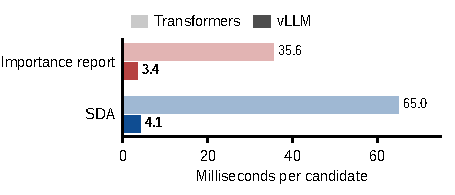
\includegraphics[width=\columnwidth]{figures/figS_serving.pdf}
\caption{Admission latency is compared for the importance report and SDA. Qwen3-8B, 1,607 original-pool candidates, one A100-80GB: milliseconds per candidate. Transformers uses one forward pass per candidate without batching; vLLM batches requests with prefix caching.}
\label{fig:appserving}
\end{figure}

\subsection{Capability with the adapter enabled on every token}
\label{app:capability}

Enabling the adapter on every token changes the four measured capability
scores by at most 0.3 percentage points under matched prompts.
Base and adapter scores are
71.6\% and 71.5\% on MMLU \citep{hendrycks2021mmlu}, 80.4\% and
80.7\% on ARC-Easy, 56.2\% and 56.4\% on ARC-Challenge
\citep{clark2018arc}, and 88.4\% and 88.6\% on the GSM8K evaluation
subset \citep{cobbe2021gsm8k}.
\FloatBarrier
\section{Answer Accuracy across Evaluation Sets and Pools}
\label{app:recall}

\subsection{Statedness-balanced pool}
\label{app:balancedresults}
Table~\ref{tab:balancedpaired} gives the paired answer accuracy differences behind \S\ref{sec:recall} for every baseline in Table~\ref{tab:balancedbaselines} and the teacher signals used directly. Table~\ref{tab:balanced} reports all six models at $k=2$ on the statedness-balanced pool: SDA exceeds each model's importance report and 1--10 importance rating. Figure~\ref{fig:appbudget} covers every budget.

\begin{table}[!htbp]
\centering
\caption{Paired SDA minus baseline answer accuracy differences (percentage points), statedness-balanced pool, Qwen3-8B, for baselines in Table~\ref{tab:balancedbaselines} and teacher signals used directly in Table~\ref{tab:balanceddirect}. Published methods: 1--10 importance rating \citep{park2023generative}; ConsistencyGate \citep{consistencygate2026}; A-MAC \citep{amac2026}; prediction error \citep{nemori2026}.}
\label{tab:balancedpaired}
\footnotesize
\setlength{\tabcolsep}{3pt}
\begin{tabular}{lccc}
\toprule
Baseline & $k=1$ & $k=2$ & $k=3$ \\
\midrule
\multicolumn{4}{l}{\emph{Importance judgments of the untrained model}} \\
Importance report & $+9.9$ & $+10.7$ & $+6.3$ \\
1--10 importance rating & $+4.7$ & $+5.2$ & $+1.1$ \\
Implied-content wording & $+9.1$ & $+9.1$ & $+4.1$ \\
\addlinespace
\multicolumn{4}{l}{\emph{Admission criteria from published methods}} \\
ConsistencyGate, sampled & $+16.5$ & $+18.7$ & $+11.0$ \\
ConsistencyGate, single pass & $+16.0$ & $+18.7$ & $+9.4$ \\
A-MAC utility & $+10.5$ & $+14.1$ & $+6.9$ \\
Prediction error & $+24.0$ & $+27.8$ & $+21.5$ \\
\addlinespace
\multicolumn{4}{l}{\emph{Statedness rules}} \\
Statedness-adjusted report & $+3.9$ & $+14.6$ & $+11.8$ \\
Reversed importance report & $+16.8$ & $+24.0$ & $+18.7$ \\
Unstated-first & $+11.8$ & $+21.8$ & $+15.4$ \\
Unstated-first with report ordering & $+3.6$ & $+14.6$ & $+11.8$ \\
\addlinespace
\multicolumn{4}{l}{\emph{Teacher signals used directly}} \\
Output likelihood used directly & $+5.8$ & $+11.8$ & $+10.2$ \\
Combined teacher used directly & $+3.6$ & $+8.8$ & $+5.5$ \\
\bottomrule
\end{tabular}
\end{table}


\begin{table*}[t]
\centering
\caption{Answer accuracy (\%) at $k=2$ across models on the statedness-balanced pool (7.93 candidates per episode).
Rating: 1--10 importance rating \citep{park2023generative}. Gold-concept selection ranks the labeled useful concept first.}
\label{tab:balanced}
\small
\setlength{\tabcolsep}{4pt}
\begin{tabular}{lccccc}
\toprule
Model & \shortstack{Importance\\report} & \shortstack{1--10\\rating} & \shortstack{Workspace\\readout} & \textbf{SDA} & \shortstack{Gold-concept\\selection} \\
\midrule
Qwen3-8B & 43.0 & 48.5 & 43.0 & \textbf{53.7} & 54.3 \\
Qwen3-14B & 35.3 & 40.0 & 36.6 & \textbf{44.1} & 46.6 \\
Qwen3-32B & 45.7 & 43.5 & 46.0 & \textbf{53.3} & 54.8 \\
Qwen2.5-7B & 23.4 & 26.4 & 24.2 & \textbf{33.3} & 31.7 \\
OLMo-2-7B & 40.5 & 47.7 & 45.2 & \textbf{54.7} & 54.8 \\
Mistral-7B & 12.7 & 16.5 & 16.2 & \textbf{19.9} & 16.8 \\
\bottomrule
\end{tabular}
\end{table*}


\begin{figure*}[t]
\centering
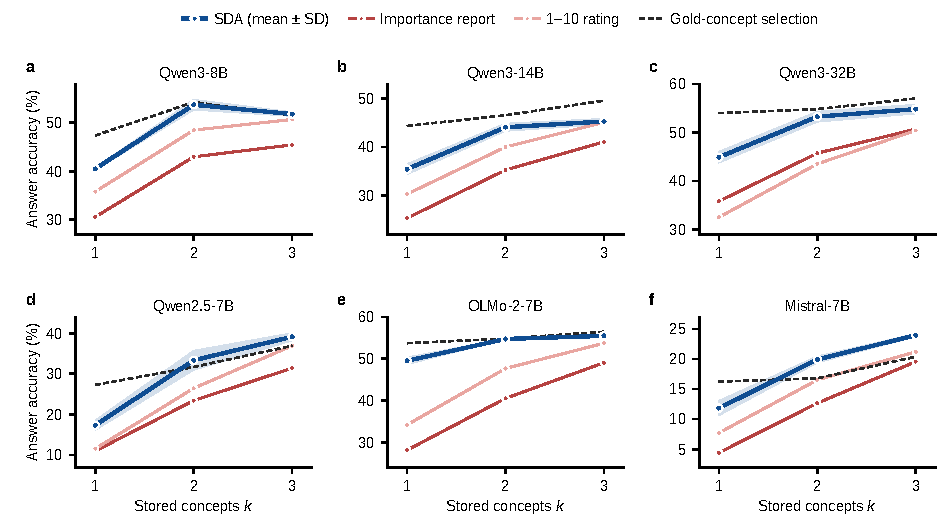
\includegraphics[width=\textwidth]{figures/figS_budget.pdf}
\caption{Admission policies are compared across memory budgets on the statedness-balanced pool. (a--f) Answer accuracy (\%) at $k=1,2,3$ stored concepts, with one model per panel.}
\label{fig:appbudget}
\end{figure*}

\subsection{Development and held-out sets}
\label{app:heldout}
Table~\ref{tab:sdamain} reports Qwen3-8B answer accuracy at $k=2$ on four development sets and the two held-out sets built with the Decoupled construction: the held-out set and the test set. SDA exceeds the importance report and matches or exceeds the 1--10 importance rating on every set.

\begin{table}[!htbp]
\centering
\caption{Qwen3-8B answer accuracy (\%) at $k=2$ on four development sets and the Decoupled held-out and test sets. Confusable and Unrelated denote Decoupled development sets with confusable or unrelated unstated distractors; $n$: number of episodes; Report: importance report; Rating: 1--10 importance rating \citep{park2023generative}; Gold: gold-concept selection.}
\label{tab:sdamain}
\small
\setlength{\tabcolsep}{4pt}
\begin{tabular}{@{}lccccc@{}}
\toprule
Set & $n$ & Report & Rating & \textbf{SDA} & Gold \\
\midrule
\multicolumn{6}{@{}l}{\emph{Development}} \\
Decoupled & 68 & 35.3 & 47.1 & \textbf{49.5} & 51.5 \\
Compositional & 52 & 46.2 & 53.8 & \textbf{54.5} & 65.4 \\
Confusable & 68 & 35.3 & \textbf{48.5} & \textbf{48.5} & 51.5 \\
Unrelated & 68 & 36.8 & 48.5 & \textbf{50.0} & 51.5 \\
\addlinespace
\multicolumn{6}{@{}l}{\emph{Held out}} \\
Held-out & 316 & 34.8 & 43.7 & \textbf{44.2} & 50.0 \\
Test & 363 & 40.8 & 45.7 & \textbf{50.0} & 54.3 \\
\bottomrule
\end{tabular}
\end{table}


\subsection{Candidate-pool comparisons}
\label{app:poolresults}
The original pool's useful concept is uniquely unstated in 95\% of episodes, and the pool with unstated distractors and the enlarged pool retain its candidates. Unstated-first with report ordering uses the importance report's strong ranking among unstated candidates, with pooled AUC 0.880--0.897 in Table~\ref{tab:withinunstated} and results in Tables~\ref{tab:baselines}, \ref{tab:bigpool} and~\ref{tab:paired}. This motivates the statedness-balanced pool, which states that concept in 190 of 363 episodes and where SDA exceeds this rule at every budget, by 14.6 points at $k=2$ (Table~\ref{tab:balancedpaired}).

\paragraph{Original pool.}
Table~\ref{tab:sdabudget} reports answer accuracy for all six models on the original pool at $k=1,2,3$: SDA exceeds each model's importance report and 1--10 importance rating in all 18 model--budget comparisons. Table~\ref{tab:baselines} reports every Qwen3-8B policy on the original pool and the pool with unstated distractors.

\begin{table}[!htbp]
\centering
\caption{Answer accuracy (\%) across models on the original pool of the test set, with $k$ stored concepts. Rep.: importance report; Rat.: 1--10 importance rating \citep{park2023generative}.}
\label{tab:sdabudget}
\small
\setlength{\tabcolsep}{2.5pt}
\resizebox{\columnwidth}{!}{%
\begin{tabular}{@{}lccccccccc@{}}
\toprule
 & \multicolumn{3}{c}{$k{=}1$} & \multicolumn{3}{c}{$k{=}2$} & \multicolumn{3}{c}{$k{=}3$} \\
\cmidrule(lr){2-4} \cmidrule(lr){5-7} \cmidrule(l){8-10}
Model & Rep. & Rat. & \textbf{SDA} & Rep. & Rat. & \textbf{SDA} & Rep. & Rat. & \textbf{SDA} \\
\midrule
Qwen3-8B & 28.1 & 34.7 & \textbf{37.6} & 40.8 & 45.7 & \textbf{50.0} & 41.6 & 47.9 & \textbf{52.2} \\
Qwen3-14B & 23.4 & 31.1 & \textbf{33.5} & 32.5 & 39.1 & \textbf{40.5} & 37.5 & 43.5 & \textbf{43.6} \\
Qwen3-32B & 32.5 & 32.0 & \textbf{41.4} & 41.0 & 44.6 & \textbf{50.2} & 46.0 & 50.7 & \textbf{53.0} \\
Qwen2.5-7B & 9.6 & 9.6 & \textbf{16.8} & 23.1 & 22.6 & \textbf{29.8} & 29.5 & 35.0 & \textbf{35.8} \\
OLMo-2-7B & 27.5 & 33.1 & \textbf{48.5} & 38.0 & 44.1 & \textbf{55.4} & 44.4 & 52.6 & \textbf{56.9} \\
Mistral-7B & 5.2 & 9.6 & \textbf{12.4} & 12.7 & 15.7 & \textbf{19.8} & 19.3 & 22.0 & \textbf{24.2} \\
\bottomrule
\end{tabular}%
}
\end{table}


\begin{table}[!htbp]
\centering
\caption{Admission policies on the original pool and pool with unstated distractors, Qwen3-8B. Answer accuracy is in
percent; rows above the rule are untrained baselines, and dashes denote unmeasured settings.}
\label{tab:baselines}
\small
\setlength{\tabcolsep}{4pt}
\resizebox{\columnwidth}{!}{%
\begin{tabular}{lcccccc}
\toprule
 & \multicolumn{3}{c}{Original pool} & \multicolumn{3}{c}{\shortstack{Pool with unstated\\distractors}} \\
\cmidrule(lr){2-4}\cmidrule(lr){5-7}
Admission policy & $k=1$ & $k=2$ & $k=3$ & $k=1$ & $k=2$ & $k=3$ \\
\midrule
Importance report & 28.1 & 40.8 & 41.6 & 28.6 & 41.0 & 41.3 \\
1--10 importance rating & 34.7 & 45.7 & 47.9 & 35.8 & 46.6 & 48.8 \\
Output likelihood & --- & 48.8 & --- & 30.6 & 39.1 & 40.5 \\
Logit-lens readout & 29.8 & 44.6 & 49.9 & 26.7 & 39.4 & 44.9 \\
\midrule
\textbf{SDA} & \textbf{37.6} & \textbf{50.0} & \textbf{52.2} & \textbf{37.6} & \textbf{50.7} & \textbf{51.6} \\
\addlinespace
\refrow Gold-concept selection & 47.1 & 54.3 & 51.5 & 47.1 & 54.3 & 51.5 \\
\bottomrule
\end{tabular}%
}

\end{table}


\paragraph{Pool with unstated distractors and enlarged pool.}
Table~\ref{tab:stress} reports answer accuracy for all six models at $k=2$ on the pool with unstated distractors: SDA exceeds each model's importance report. Table~\ref{tab:bigpool} reports Qwen3-8B on the enlarged pool: SDA exceeds the importance report, output likelihood and workspace readout at every budget. Table~\ref{tab:paired} gives paired SDA minus baseline differences on the three pools.

\begin{table}[!htbp]
\centering
\caption{Answer accuracy (\%) across models on the pool with unstated distractors
(test set, 8.42 candidates per episode) at $k=2$, with SDA values
averaged over three training runs.}
\label{tab:stress}
\small
\setlength{\tabcolsep}{4pt}
\begin{tabular}{lccc}
\toprule
Model & Importance report & \textbf{SDA} & \shortstack{Gold-concept\\selection} \\
\midrule
Qwen3-8B & 41.0 & \textbf{50.7} & 54.3 \\
Qwen3-14B & 32.2 & \textbf{40.0} & 46.6 \\
Qwen3-32B & 41.0 & \textbf{50.6} & 54.8 \\
Qwen2.5-7B & 23.7 & \textbf{30.1} & 31.7 \\
OLMo-2-7B & 38.8 & \textbf{51.5} & 54.8 \\
Mistral-7B & 12.9 & \textbf{18.8} & 16.8 \\
\bottomrule
\end{tabular}

\end{table}


\begin{table*}[t]
\centering
\caption{Answer accuracy (\%) on the enlarged pool (confirmation set, 12.41 candidates per episode), Qwen3-8B. }
\label{tab:bigpool}
\small
\setlength{\tabcolsep}{3pt}
\begin{tabular}{lccccc}
\toprule
Budget & \shortstack{Importance\\report} & \shortstack{Output\\likelihood} & \shortstack{Workspace\\readout} & \textbf{SDA} & \shortstack{Gold-concept\\selection} \\
\midrule
$k=1$ & 29.5 & 28.1 & 24.0 & \textbf{38.6} & 47.1 \\
$k=2$ & 40.5 & 32.0 & 34.7 & \textbf{51.5} & 54.3 \\
$k=3$ & 41.9 & 33.9 & 38.6 & \textbf{52.3} & 51.5 \\
\bottomrule
\end{tabular}

\end{table*}


\begin{table*}[t]
\centering
\caption{Paired SDA minus baseline answer-accuracy differences on three candidate pools, Qwen3-8B. Entries are in
percentage points.}
\label{tab:paired}
\small
\setlength{\tabcolsep}{3pt}
\begin{tabular}{lccc}
\toprule
Baseline & $k=1$ & $k=2$ & $k=3$ \\
\midrule
\multicolumn{4}{l}{\emph{Original pool}} \\
\quad Importance report & $+9.6$ & $+9.3$ & $+10.6$ \\
\quad 1--10 importance rating & $+2.9$ & $+4.3$ & $+4.2$ \\
\quad Statedness-cued wording & $+5.4$ & $+7.1$ & $+6.2$ \\
\quad Reversed importance report & $+2.1$ & $+3.5$ & $+3.1$ \\
\quad Unstated-first & $-8.9$ & $-3.4$ & $+2.6$ \\
\quad Unstated-first with report ordering & $-9.5$ & $-3.4$ & $-0.5$ \\
\quad Random selection & $+9.0$ & $+5.4$ & $+5.6$ \\
\addlinespace
\multicolumn{4}{l}{\emph{Pool with unstated distractors}} \\
\quad Importance report & $+8.9$ & $+9.6$ & $+10.3$ \\
\quad 1--10 importance rating & $+1.7$ & $+4.1$ & $+2.9$ \\
\quad Reversed importance report & $+14.1$ & $+21.8$ & $+20.8$ \\
\quad Unstated-first & $+5.9$ & $+15.4$ & $+14.7$ \\
\quad Unstated-first with report ordering & $-8.4$ & $+5.8$ & $+8.9$ \\
\quad Output likelihood & $+7.0$ & $+11.6$ & $+11.1$ \\
\addlinespace
\multicolumn{4}{l}{\emph{Enlarged pool}} \\
\quad Importance report & $+9.1$ & $+11.0$ & $+10.5$ \\
\quad 1--10 importance rating & $+2.2$ & $+4.7$ & $+4.1$ \\
\quad Unstated-first with report ordering & $-5.5$ & $+6.6$ & $+12.1$ \\
\quad Output likelihood & $+10.5$ & $+19.6$ & $+18.5$ \\
\quad Random selection & $+17.1$ & $+24.5$ & $+22.6$ \\
\bottomrule
\end{tabular}

\end{table*}


\paragraph{Naming-balanced pool.}
Table~\ref{tab:namingrecall} reports answer accuracy for all six models at $k=1,2,3$: SDA exceeds each model's importance report in 17 of 18 comparisons, trailing by 0.1 points otherwise, and the 1--10 importance rating in all twelve comparisons at $k=1,2$.
SDA improves ranking and retention under the naming-balanced construction
(Table~\ref{tab:namingbalanced}). For Qwen3-8B, within-episode
AUC is 0.722, versus 0.566 for the report and 0.636 for the
workspace readout. Useful-concept retention at $k=2$ is 53.7\%,
versus 24.0\% and 40.8\%, respectively.

\begin{table*}[t]
\centering
\caption{Answer accuracy (\%) on the naming-balanced pool, six models, at one, two and three stored concepts. Report:
each model's importance report; Rating: 1--10 importance rating
\citep{park2023generative}.}
\label{tab:namingrecall}
\small
\setlength{\tabcolsep}{3.5pt}
\begin{tabular}{lccccccccc}
\toprule
& \multicolumn{3}{c}{$k=1$} & \multicolumn{3}{c}{$k=2$} & \multicolumn{3}{c}{$k=3$} \\
\cmidrule(lr){2-4} \cmidrule(lr){5-7} \cmidrule(lr){8-10}
Model & Report & Rating & \textbf{SDA} & Report & Rating & \textbf{SDA} & Report & Rating & \textbf{SDA} \\
\midrule
Qwen3-8B & 27.6 & 35.3 & \textbf{36.4} & 42.7 & 45.2 & \textbf{46.2} & 46.3 & 47.1 & \textbf{47.0} \\
Qwen3-14B & 21.8 & 30.3 & \textbf{33.7} & 33.3 & 36.4 & \textbf{40.8} & 41.3 & 43.2 & \textbf{41.2} \\
Qwen3-32B & 31.7 & 30.0 & \textbf{41.1} & 43.2 & 43.0 & \textbf{48.9} & 50.7 & 51.8 & \textbf{53.4} \\
Qwen2.5-7B & 9.4 & 11.6 & \textbf{13.3} & 21.2 & 25.6 & \textbf{28.3} & 28.6 & 33.3 & \textbf{33.0} \\
OLMo-2-7B & 24.8 & 30.6 & \textbf{37.0} & 39.4 & 43.0 & \textbf{46.7} & 44.6 & 52.1 & \textbf{49.5} \\
Mistral-7B & 4.7 & 5.8 & \textbf{9.9} & 9.6 & 13.2 & \textbf{16.0} & 19.8 & 21.5 & \textbf{23.7} \\
\bottomrule
\end{tabular}
\end{table*}


\begin{table}[!htbp]
\centering
\caption{Candidate ranking and useful-concept retention on the naming-balanced pool, Qwen3-8B, 2,877
candidates. Entries are AUC and retention (\%).}
\label{tab:namingbalanced}
\small
\setlength{\tabcolsep}{4pt}
\resizebox{\columnwidth}{!}{%
\begin{tabular}{lccccc}
\toprule
Admission policy & \shortstack{Pooled\\AUC} & \shortstack{Within-episode\\AUC} & $B_1$ & $B_2$ & $B_3$ \\
\midrule
Importance report & 0.570 & 0.566 & 9.4 & 24.0 & 42.7 \\
Logit-lens readout & 0.635 & 0.636 & 22.0 & 40.8 & 54.8 \\
\textbf{SDA} & \textbf{0.723} & \textbf{0.722} & \textbf{34.6} & \textbf{53.7} & \textbf{67.0} \\
\bottomrule
\end{tabular}%
}
\end{table}


\subsection{Within-episode ranking and useful-concept retention}
\label{app:episodemetrics}

SDA improves both within-episode ranking and retention of the useful
concept at $k=2$ (Table~\ref{tab:episodemetrics}).
Conditional accuracy separates retaining the useful concept from
answering the question: for the reference SDA training run, accuracy is
54.6\% when the useful concept is retained and 41.2\% when it is not,
versus 48.2\% and 37.7\% for the report.

\begin{table*}[t]
\centering
\caption{Within-episode admission ranking on the original pool, Qwen3-8B. AUC differences are
relative to the importance report; retention (\%) measures whether the two admitted concepts
include the useful concept.}
\label{tab:episodemetrics}
\small
\setlength{\tabcolsep}{4pt}
\begin{tabular}{lccc}
\toprule
Admission score & \shortstack{Within-episode AUC} & \shortstack{$\Delta$ vs.\ report} & \shortstack{Useful concept\\retained ($k=2$)} \\
\midrule
Importance report & 0.326 & \emph{reference} & 29.8 \\
1--10 importance rating \citep{park2023generative} & 0.608 & $+0.282$ & 61.2 \\
Workspace readout & 0.547 & $+0.221$ & 51.0 \\
Output likelihood & 0.619 & $+0.293$ & 59.2 \\
\textbf{SDA} & \textbf{0.683} & $+0.357$ & \textbf{69.1} \\
\bottomrule
\end{tabular}

\end{table*}


\paragraph{Gold-concept selection and answer accuracy.}
Qwen3-8B reaches 54.3\% answer accuracy with gold-concept selection and
50.0\% with SDA. The reader answers from the complete stored set and
its own knowledge. On OLMo-2-7B and Mistral-7B, SDA reaches 55.4\% and
19.8\%, versus 54.8\% and 16.8\% for gold-concept selection (Tables~\ref{tab:sdabudget} and~\ref{tab:balanced}).
\FloatBarrier
\section{Statedness and Wording Measurements}
\label{app:provenance}

\subsection{Ranking among candidates with the same statedness}
\label{app:withinprovenance}

Restricting the pool with unstated distractors to episodes with an
unstated useful concept and at least one unstated negative leaves
345 episodes, with 5.01 qualifying candidates per episode on average.
\S\ref{sec:gap} reports the resulting AUCs
(Table~\ref{tab:withinunstated}).
This measurement holds statedness fixed; the full-pool comparison
measures the competition between stated and unstated candidates.

\begin{table}[H]
\centering
\caption{Useful-concept ranking among unstated candidates, pool with unstated distractors. Qualifying
episodes (345) average 5.01 candidates, including unstated useful and negative concepts. Entries:
pooled AUC; $R-V$: logit-lens readout minus importance report.}
\label{tab:withinunstated}
\small
\setlength{\tabcolsep}{5pt}
\resizebox{\columnwidth}{!}{%
\begin{tabular}{lccc}
\toprule
Model & Importance report & Logit-lens readout & $R-V$ \\
\midrule
Qwen3-8B & 0.881 & 0.639 & $-0.242$ \\
Qwen3-14B & 0.880 & 0.654 & $-0.226$ \\
Qwen3-32B & 0.896 & 0.697 & $-0.199$ \\
Qwen2.5-7B & 0.897 & 0.592 & $-0.305$ \\
OLMo-2-7B & 0.883 & 0.661 & $-0.221$ \\
Mistral-7B & 0.880 & 0.672 & $-0.208$ \\
\bottomrule
\end{tabular}%
}
\end{table}


\subsection{Importance wordings}
\label{app:wording}

Five matched wordings keep the episode, candidates and gold utility labels fixed. They ask about passage-only importance, remove that restriction, allow implied content (\emph{implied-content wording}), state that the passage may omit the useful concept (\emph{statedness-cued wording}), or specify a two-concept budget. Each replaces the importance prompt's question and is scored with Eq.~\eqref{eq:score} using the same token sets and thinking-disabled prompt as the importance report (App.~\ref{app:prompts}). The passage-only wording is the importance prompt, so its row is the importance report. Table~\ref{tab:wordingtext} gives each question; it follows the passage, and \emph{candidate} is replaced by the candidate concept.

Wording effects vary in direction and magnitude across four models on the original pool and the pool with unstated distractors (Table~\ref{tab:wording}). The statedness-cued wording raises original-pool pooled AUC from 0.398 to 0.877 for Qwen3-32B and 0.322 to 0.527 for Qwen3-8B; the implied-content wording raises it from 0.411 to 0.456 for Mistral-7B. In 95\% of original-pool episodes, the useful concept is the sole unstated candidate (App.~\ref{app:pools}), so favoring unstated candidates raises AUC.

The statedness-cued wording reverses Qwen3-8B's preference, favoring unstated candidates: against the importance report, pooled AUC rises on the original pool (0.527 versus 0.322) and falls on the stated-bridge control (0.410 versus 0.515) and the 88 Explicit episodes (0.621 versus 0.710), whose passages state the useful concept.

Both wordings stay close to the importance report on the statedness-balanced pool for Qwen3-8B: at $k=1,2,3$, answer accuracy is 31.7\%, 44.9\%, 47.7\% for the implied-content wording and 31.4\%, 42.7\%, 45.5\% for the statedness-cued wording, versus 30.6\%, 43.0\%, 45.5\%. SDA exceeds each at every budget with 40.5\%, 53.7\%, 51.8\% (Tables~\ref{tab:balancedbaselines} and~\ref{tab:balancedpaired}). On the original pool, the statedness-cued wording reaches 31.4\%, 43.8\%, 46.0\%, each 6.2 points below SDA (Table~\ref{tab:paired}).

The implied-content wording permits inferences without specifying whether the passage states the useful concept, and the matched comparison trains and evaluates SDA through it. Original-pool answer accuracy on Qwen3-8B rises from the importance report's 28.1\%, 40.8\% and 41.6\% to 30.6\%, 42.1\% and 44.9\% at $k=1,2,3$. SDA exceeds it at every budget, reaching 37.1\%, 50.7\% and 51.0\% (Table~\ref{tab:wordingdistill}).

\begin{table*}[t]
\centering
\caption{Implied-content wording and distillation on the standard pool, Qwen3-8B. Answer accuracy is in percent; the
final row gives answer-accuracy differences in points.}
\label{tab:wordingdistill}
\small
\setlength{\tabcolsep}{4pt}
\begin{tabular}{lccc}
\toprule
Admission policy & $k=1$ & $k=2$ & $k=3$ \\
\midrule
Importance report & 28.1 & 40.8 & 41.6 \\
Implied-content wording & 29.2 & 41.3 & 44.9 \\
\textbf{SDA with implied-content wording} & \textbf{37.1} & \textbf{50.7} & \textbf{51.0} \\
SDA minus implied-content wording & $+7.9$ & $+9.4$ & $+6.1$ \\
\bottomrule
\end{tabular}

\end{table*}

\begin{table}[!htbp]
\centering
\caption{Qwen3-8B pooled useful-concept AUC under three matched importance prompt wordings on the original pool and the pool with unstated distractors.}
\label{tab:wording}
\small
\setlength{\tabcolsep}{3pt}
\begin{tabular}{@{}lcc@{}}
\toprule
Importance wording & Original pool & \shortstack{Pool with unstated\\distractors} \\
\midrule
Passage only & 0.322 & 0.627 \\
Implied-content wording & 0.461 & 0.692 \\
Statedness-cued wording & 0.527 & 0.722 \\
\bottomrule
\end{tabular}
\end{table}

\begin{table}[!htbp]
\centering
\caption{Questions for the three matched importance prompt wordings evaluated with Qwen3-8B. Each question follows the passage, with \emph{candidate} replaced by the candidate concept.}
\label{tab:wordingtext}
\small
\setlength{\tabcolsep}{6pt}
\begin{tabular}{@{}p{0.27\columnwidth}p{0.67\columnwidth}@{}}
\toprule
Wording & Question \\
\midrule
Passage only & Based only on the passage above, is the concept \emph{candidate} one of the most important things to remember in order to answer possible future questions? Answer with a single word: yes or no. \\
\addlinespace
Implied-content wording & Considering both what the passage above states and what it implies without stating, is the concept \emph{candidate} one of the most important things to remember in order to answer possible future questions? Answer with a single word: yes or no. \\
\addlinespace
Statedness-cued wording & Would storing the concept \emph{candidate} help answer a likely future question about the passage above, even if the passage never mentions it? Answer with a single word: yes or no. \\
\bottomrule
\end{tabular}
\end{table}


\subsection{Matched naming and position measurements}
\label{app:naming}

Naming the useful concept raises both teacher signals more than
the importance report or the 1--10 importance rating on Qwen3-8B.
Workspace, output likelihood, report and rating AUCs on the original
passage are 0.543, 0.613, 0.322 and 0.568. Appending a sentence naming
the useful concept (the named condition) raises them to 0.952, 0.859,
0.515 and 0.581; placing the same sentence before the passage yields
0.916, 0.850, 0.582 and 0.655.
Naming a distractor instead yields 0.393, 0.520, 0.249 and 0.519.
Table~\ref{tab:statedcontrol} gives the six-model results summarized
in \S\ref{sec:gap}. The six individual report
changes include Mistral-7B's change from 0.411 to 0.395.

\begin{table*}[t]
\centering
\caption{Stated-bridge control on the original pool: original passage versus passage with one added sentence naming the useful concept. Entries: pooled AUC; $W$:
logit-lens readout; $\mathrm{LL}$: output likelihood; Report: importance report; Rating: 1--10
importance rating.}
\label{tab:statedcontrol}
\small
\setlength{\tabcolsep}{4pt}
\begin{tabular}{lcccccccc}
\toprule
& \multicolumn{2}{c}{$W$} & \multicolumn{2}{c}{$\mathrm{LL}$} & \multicolumn{2}{c}{Report} & \multicolumn{2}{c}{Rating} \\
\cmidrule(lr){2-3}\cmidrule(lr){4-5}\cmidrule(lr){6-7}\cmidrule(lr){8-9}
Model & Original & Named & Original & Named & Original & Named & Original & Named \\
\midrule
Qwen3-8B & 0.543 & 0.952 & 0.613 & 0.859 & 0.322 & 0.515 & 0.568 & 0.581 \\
Qwen3-14B & 0.571 & 0.954 & 0.636 & 0.864 & 0.355 & 0.607 & 0.565 & 0.591 \\
Qwen3-32B & 0.603 & 0.979 & 0.654 & 0.878 & 0.398 & 0.638 & 0.530 & 0.510 \\
Qwen2.5-7B & 0.520 & 0.879 & 0.600 & 0.890 & 0.427 & 0.456 & 0.481 & 0.481 \\
OLMo-2-7B & 0.561 & 0.986 & 0.633 & 0.911 & 0.327 & 0.410 & 0.533 & 0.585 \\
Mistral-7B & 0.581 & 0.990 & 0.630 & 0.854 & 0.411 & 0.395 & 0.608 & 0.601 \\
\midrule
Mean & 0.563 & 0.956 & 0.628 & 0.876 & 0.373 & 0.504 & 0.548 & 0.558 \\
\bottomrule
\end{tabular}
\end{table*}


On the stated-bridge control at $k=2$, SDA reaches 54.6\% answer accuracy, against 44.9\% for the report and 39.9\% for the reversed importance report.
\FloatBarrier
\section{Extended Ranking Measurements}
\label{app:measurements}

\subsection{Alternate-generator and entity-bridge sets}
\label{app:replications}

The report's preference for stated candidates persists with a different
generator. Across six models on the alternate-generator set,
report AUC ranges from 0.220 to 0.384, alongside statedness AUC
0.650--0.803 (Table~\ref{tab:replications}). These measurements use
the same report definition as the GPT-4.1 sets. The alternate-generator
set also supplies SDA training episodes, so these untrained-model
measurements replicate the diagnostic rather than evaluate SDA.

\begin{table}[!htbp]
\centering
\caption{Pooled useful-concept AUC and the importance report's statedness AUC for six unadapted models on the alternate-generator set. $R$: logit-lens readout; $V$: importance report.}
\label{tab:replications}
\small
\setlength{\tabcolsep}{5pt}
\begin{tabular}{@{}lcccc@{}}
\toprule
Model & $R$ & $V$ & $R-V$ & Statedness AUC \\
\midrule
Qwen3-8B & 0.515 & 0.220 & $+0.295$ & 0.803 \\
Qwen3-14B & 0.521 & 0.267 & $+0.254$ & 0.754 \\
Qwen3-32B & 0.522 & 0.275 & $+0.247$ & 0.758 \\
Qwen2.5-7B & 0.490 & 0.384 & $+0.106$ & 0.650 \\
OLMo-2-7B & 0.547 & 0.353 & $+0.194$ & 0.668 \\
Mistral-7B & 0.507 & 0.294 & $+0.213$ & 0.700 \\
\bottomrule
\end{tabular}
\end{table}


\paragraph{Entity-bridge set.}
The set places a named-entity useful concept among scene-object distractors. Qwen2.5-7B and Qwen3-8B importance reports prefer unstated candidates (statedness AUCs 0.133, 0.289); their importance report AUCs (0.881, 0.719) exceed workspace readout AUCs (0.664, 0.642). Qwen2.5-0.5B's importance report prefers stated candidates (statedness AUC 0.734; importance report AUC 0.270). The statedness preference follows set construction. Passage replacement lowers Qwen2.5-7B and Qwen3-8B importance report AUCs to 0.282 and 0.340, showing dependence on each episode's own passage. SDA reaches pooled AUC 0.985 and within-episode AUC 1.000; the reversed importance report reaches 0.281. Reversal helps only when the importance report prefers stated candidates and the useful concept is unstated.

\subsection{Admission after distillation across scales}
\label{app:sdascale}

SDA raises pooled AUC on the development sets at every measured Qwen3
scale (Table~\ref{tab:sdascale}).
The measured improvement is concentrated in the admission score, while
the largest absolute workspace AUC change is 0.0046.

\begin{table}[!htbp]
\centering
\caption{Admission ranking on the Decoupled and Compositional development sets
across Qwen3 scales, with one row per model and set. $V$: pooled AUC
of the admission score (untrained before, SDA after). $V$ after is the
mean over three training runs; $\Delta V$: change of that mean;
$|\Delta W|$: largest absolute workspace readout change across the
three training runs.}
\label{tab:sdascale}
\small
\setlength{\tabcolsep}{4pt}
\resizebox{\columnwidth}{!}{%
\begin{tabular}{llcccc}
\toprule
Model & Set & $V$ before & $V$ after & $\Delta V$ & $|\Delta W|$ \\
\midrule
Qwen3-8B & Decoupled & 0.387 & \textbf{0.751} & $+0.364$ & 0.0033 \\
Qwen3-8B & Compositional & 0.208 & \textbf{0.620} & $+0.412$ & 0.0021 \\
Qwen3-14B & Decoupled & 0.427 & \textbf{0.683} & $+0.256$ & 0.0029 \\
Qwen3-14B & Compositional & 0.216 & \textbf{0.489} & $+0.273$ & 0.0029 \\
Qwen3-32B & Decoupled & 0.478 & \textbf{0.752} & $+0.274$ & 0.0037 \\
Qwen3-32B & Compositional & 0.277 & \textbf{0.611} & $+0.334$ & 0.0046 \\
\bottomrule
\end{tabular}%
}

\end{table}


\FloatBarrier
\section{Teacher and Optimization Measurements}
\label{app:ablations}

\subsection{Teacher composition and workspace readout}

\label{app:teacherreadout}

Table~\ref{tab:teachermodels} reports answer accuracy on the
statedness-balanced pool for all three teacher compositions. Table~\ref{tab:teacherretention} splits the comparison by statedness
condition and reports retention as well as answer accuracy for five
models.
In the unstated-concept condition, removing the workspace readout lowers
retention in all five models at every budget, by an average of 6.6, 4.5
and 2.5 points at $k=1,2,3$, and lowers mean answer accuracy by 1.8 and
0.8 points at $k=1,2$, whereas removing output likelihood changes mean
retention by at most 0.8 points.
Section~\ref{sec:ablations} relates these retention differences to
answer accuracy.

\begin{table}[H]
\centering
\caption{Teacher composition on the statedness-balanced pool, five models. Answer accuracy (\%); the two ``Without'' columns show
students trained with one teacher signal removed.}
\label{tab:teachermodels}
\small
\setlength{\tabcolsep}{4pt}
\resizebox{\columnwidth}{!}{%
\begin{tabular}{llccc}
\toprule
Model & Budget & \textbf{SDA} & \shortstack{Without the\\logit-lens readout} & \shortstack{Without the\\output likelihood} \\
\midrule
Qwen3-8B & $k=1$ & 40.5 & \textbf{42.1} & 36.7 \\
 & $k=2$ & 53.7 & \textbf{54.8} & 49.8 \\
 & $k=3$ & \textbf{51.8} & 50.6 & 50.5 \\
\addlinespace
Qwen3-14B & $k=1$ & 35.5 & \textbf{36.2} & 34.3 \\
 & $k=2$ & \textbf{44.1} & 43.4 & 42.4 \\
 & $k=3$ & 45.3 & \textbf{45.8} & 45.2 \\
\addlinespace
Qwen3-32B & $k=1$ & 44.9 & 43.4 & \textbf{45.7} \\
 & $k=2$ & 53.3 & 52.2 & \textbf{54.7} \\
 & $k=3$ & 54.8 & 55.3 & \textbf{56.6} \\
\addlinespace
Qwen2.5-7B & $k=1$ & 17.4 & 16.2 & \textbf{17.6} \\
 & $k=2$ & \textbf{33.3} & 32.2 & 32.4 \\
 & $k=3$ & \textbf{39.1} & 37.6 & 37.3 \\
\addlinespace
OLMo-2-7B & $k=1$ & \textbf{49.5} & 46.2 & 45.2 \\
 & $k=2$ & \textbf{54.7} & 53.4 & 51.1 \\
 & $k=3$ & \textbf{55.5} & \textbf{55.5} & 55.2 \\
\bottomrule
\end{tabular}%
}
\end{table}


\begin{table}[!htbp]
\centering
\caption{Teacher-signal ablations on stated and implied episodes of the statedness-balanced pool across five models. Entries are SDA minus the
student trained without the named signal, in percentage points
(positive: removing the signal lowers the quantity); averages over
the five models and three training runs. Models: number of the five models whose difference is positive.}
\label{tab:teacherretention}
\small
\setlength{\tabcolsep}{4pt}
\resizebox{\columnwidth}{!}{%
\begin{tabular}{llccccc}
\toprule
 & & \multicolumn{3}{c}{\shortstack{Without the\\logit-lens readout}} & \multicolumn{2}{c}{\shortstack{Without the\\output likelihood}} \\
\cmidrule(lr){3-5}\cmidrule(lr){6-7}
Episodes & Budget & Ret. & Models & Acc. & Ret. & Acc. \\
\midrule
Implied (173) & $k=1$ & $+6.6$ & 5/5 & $+1.8$ & $-0.8$ & $+0.5$ \\
 & $k=2$ & $+4.5$ & 5/5 & $+0.8$ & $+0.5$ & $+1.5$ \\
 & $k=3$ & $+2.5$ & 5/5 & $-0.1$ & $0.0$ & $+0.6$ \\
\addlinespace
Stated (190) & $k=1$ & $-0.6$ & 3/5 & $-0.3$ & $+2.2$ & $+2.7$ \\
 & $k=2$ & $+0.9$ & 4/5 & $+0.4$ & $+1.9$ & $+2.0$ \\
 & $k=3$ & $+0.5$ & 3/5 & $+0.7$ & $+1.8$ & $+0.1$ \\
\addlinespace
All (363) & $k=1$ & $+2.8$ & 4/5 & $+0.7$ & $+0.8$ & $+1.6$ \\
 & $k=2$ & $+2.6$ & 4/5 & $+0.6$ & $+1.2$ & $+1.7$ \\
 & $k=3$ & $+1.4$ & 4/5 & $+0.3$ & $+0.9$ & $+0.3$ \\
\bottomrule
\end{tabular}%
}
\end{table}


\subsection{Paired-passage set}
\label{app:pairedresults}
Table~\ref{tab:crosspairpooled} pools the paired-passage set results over the five models, Table~\ref{tab:crosspairmodels} gives them per model, and App.~\ref{app:pairedpassage} describes the set.

\begin{table}[!htbp]
\centering
\caption{Paired-passage set results for Qwen3-8B, Qwen3-14B, Qwen3-32B, Qwen2.5-7B and OLMo-2-7B.
Entries: SDA minus students trained with one teacher signal removed, pooled across models, in
percentage points; retention indicates admission of the useful concept.}
\label{tab:crosspairpooled}
\small
\setlength{\tabcolsep}{4pt}
\resizebox{\columnwidth}{!}{%
\begin{tabular}{lcccc}
\toprule
& \multicolumn{2}{c}{Without the workspace readout} & \multicolumn{2}{c}{Without the output likelihood} \\
\cmidrule(lr){2-3}\cmidrule(lr){4-5}
Budget & Retention & Accuracy & Retention & Accuracy \\
\midrule
$k=1$ & $+7.3$ & $+1.9$ & $-1.4$ & $+1.3$ \\
$k=2$ & $+4.6$ & $+0.6$ & $+0.1$ & $+1.6$ \\
$k=3$ & $+3.0$ & $+1.1$ & $+1.7$ & $+1.4$ \\
\bottomrule
\end{tabular}%
}
\end{table}


\begin{table*}[t]
\centering
\caption{Paired-passage set results by model. Entries are SDA minus students trained with one teacher
signal removed, in percentage points; retention indicates admission of the episode's useful concept.}
\label{tab:crosspairmodels}
\footnotesize
\setlength{\tabcolsep}{2pt}
\begin{tabular}{llcccc}
\toprule
& & \multicolumn{2}{c}{Without the logit-lens readout} & \multicolumn{2}{c}{Without the output likelihood} \\
\cmidrule(lr){3-4}\cmidrule(lr){5-6}
Model & Budget & Retention & Accuracy & Retention & Accuracy \\
\midrule
Qwen3-8B & $k=1$ & $+5.3$ & $-0.1$ & $+2.9$ & $+3.0$ \\
 & $k=2$ & $+3.1$ & $-0.2$ & $+2.4$ & $+3.2$ \\
 & $k=3$ & $+3.5$ & $+1.7$ & $+2.2$ & $+2.3$ \\
\addlinespace
Qwen3-14B & $k=1$ & $+9.0$ & $+1.4$ & $-1.4$ & $+0.3$ \\
 & $k=2$ & $+6.0$ & $+0.0$ & $-1.3$ & $+1.3$ \\
 & $k=3$ & $+2.3$ & $+0.6$ & $+1.6$ & $+1.8$ \\
\addlinespace
Qwen3-32B & $k=1$ & $+3.8$ & $+1.6$ & $-10.6$ & $-1.9$ \\
 & $k=2$ & $+1.8$ & $+0.7$ & $-6.2$ & $-0.3$ \\
 & $k=3$ & $+0.7$ & $+0.2$ & $-4.5$ & $-0.8$ \\
\addlinespace
Qwen2.5-7B & $k=1$ & $+8.3$ & $+3.0$ & $-1.6$ & $+0.8$ \\
 & $k=2$ & $+6.2$ & $+1.8$ & $+0.6$ & $+0.6$ \\
 & $k=3$ & $+4.4$ & $+1.5$ & $+4.3$ & $+0.4$ \\
\addlinespace
OLMo-2-7B & $k=1$ & $+10.0$ & $+3.4$ & $+3.9$ & $+4.4$ \\
 & $k=2$ & $+6.0$ & $+0.7$ & $+5.0$ & $+3.1$ \\
 & $k=3$ & $+4.0$ & $+1.7$ & $+4.8$ & $+3.4$ \\
\bottomrule
\end{tabular}
\end{table*}


\subsection{Passage replacement}
\label{app:context}
Passage replacement assigns each episode another episode's passage under a fixed permutation, preserving candidates, labels and question. For untrained signals (Table~\ref{tab:readoutshuffle}), workspace readout AUC falls across all six models, from 0.543 to 0.433 on Qwen3-8B and from 0.581 to 0.423 on Mistral-7B. Qwen3-8B output likelihood AUC changes from 0.613 to 0.604 and importance report AUC from 0.322 to 0.485. Output likelihood retains a context-independent candidate prior; the workspace readout and the importance report's preference for stated candidates depend on the episode's own passage. SDA's within-episode AUC falls from 0.683 to 0.544 (pooled AUC 0.538). Table~\ref{tab:replacedpassage} gives Qwen3-8B useful-concept retention measurements behind Figure~\ref{fig:mechanism}c, alongside the untrained workspace readout and importance report. All importance report measurements use Eq.~\eqref{eq:score} and the importance prompt (App.~\ref{app:prompts}).

\begin{table}[!htbp]
\centering
\caption{Pooled useful-concept AUC of the logit-lens readout for six models on the original pool with each episode's own passage or another episode's passage.}
\label{tab:readoutshuffle}
\small
\setlength{\tabcolsep}{5pt}
\begin{tabular}{@{}lcc@{}}
\toprule
Model & Own passage & Replaced passage \\
\midrule
Qwen3-8B & 0.543 & 0.433 \\
Qwen3-14B & 0.571 & 0.473 \\
Qwen3-32B & 0.602 & 0.479 \\
Qwen2.5-7B & 0.520 & 0.509 \\
OLMo-2-7B & 0.561 & 0.477 \\
Mistral-7B & 0.581 & 0.423 \\
\bottomrule
\end{tabular}
\end{table}


\begin{table}[!htbp]
\centering
\caption{Passage replacement on the original pool, Qwen3-8B. Retention (\%) measures whether the
single stored concept is useful; drops are own-passage retention minus retention with another
episode's passage.}
\label{tab:replacedpassage}
\small
\setlength{\tabcolsep}{5pt}
\resizebox{\columnwidth}{!}{%
\begin{tabular}{lccc}
\toprule
Admission policy & Own passage & Replaced passage & Drop \\
\midrule
\textbf{SDA} & 48.3 & 27.4 & $+20.9$ \\
Without the logit-lens readout & 42.8 & 39.9 & $+2.9$ \\
Without the output likelihood & 46.6 & 20.1 & $+26.5$ \\
Logit-lens readout & 26.2 & 14.3 & $+11.8$ \\
Importance report & 16.0 & 20.4 & $-4.4$ \\
\bottomrule
\end{tabular}%
}
\end{table}


\subsection{Teacher signals used directly}
\label{app:direct}
Ranking directly by teacher signals without training an adapter yields lower answer accuracy than SDA. On the statedness-balanced pool, Qwen3-8B's combined teacher reaches 36.9\%, 44.9\%, 46.3\% and output likelihood 34.7\%, 41.9\%, 41.6\%, against SDA's 40.5\%, 53.7\%, 51.8\% at $k=1,2,3$ (Table~\ref{tab:balanceddirect}; paired differences: Table~\ref{tab:balancedpaired}). On the original pool at $k=2$, the combined teacher reaches 45.7\%, 4.3 points below SDA; the workspace readout reaches 44.6\%, 5.4 points below; and output likelihood reaches 48.8\%, 1.3 points below (Tables~\ref{tab:sdaablation} and~\ref{tab:baselines}).

\begin{table}[t]
\centering
\caption{Qwen3-8B answer accuracy (\%) on the statedness-balanced pool at $k=1,2,3$: SDA and ranking directly by the combined teacher or output likelihood without training an adapter.}
\label{tab:balanceddirect}
\small
\setlength{\tabcolsep}{4pt}
\begin{tabular}{lccc}
\toprule
Admission policy & $k=1$ & $k=2$ & $k=3$ \\
\midrule
\textbf{SDA} & \textbf{40.5} & \textbf{53.7} & \textbf{51.8} \\
Combined teacher used directly & 36.9 & 44.9 & 46.3 \\
Output likelihood used directly & 34.7 & 41.9 & 41.6 \\
\bottomrule
\end{tabular}
\end{table}


\begin{table}[!htbp]
\centering
\caption{SDA ablations on the original pool, Qwen3-8B, $k=2$. Answer accuracy is in percent; $\Delta$ is the
accuracy difference from SDA in percentage points.}
\label{tab:sdaablation}
\small
\setlength{\tabcolsep}{5pt}
\resizebox{\columnwidth}{!}{%
\begin{tabular}{lcc}
\toprule
Variant & Accuracy & $\Delta$ vs.\ SDA \\
\midrule
\textbf{SDA} & \textbf{50.0} & \emph{reference} \\
\addlinespace
\multicolumn{3}{l}{\emph{No distillation}} \\
Combined teacher used directly & 45.7 & $-4.3$ \\
\addlinespace
\multicolumn{3}{l}{\emph{Accuracy reward}} \\
Accuracy reward instead of distillation & 46.4 & $-3.7$ \\
SDA followed by accuracy-reward refinement & 52.9 & $+2.8$ \\
\bottomrule
\end{tabular}%
}
\end{table}


\subsection{Accuracy reward}
\label{app:ablationprotocol}
\begin{figure}[!htbp]
\centering
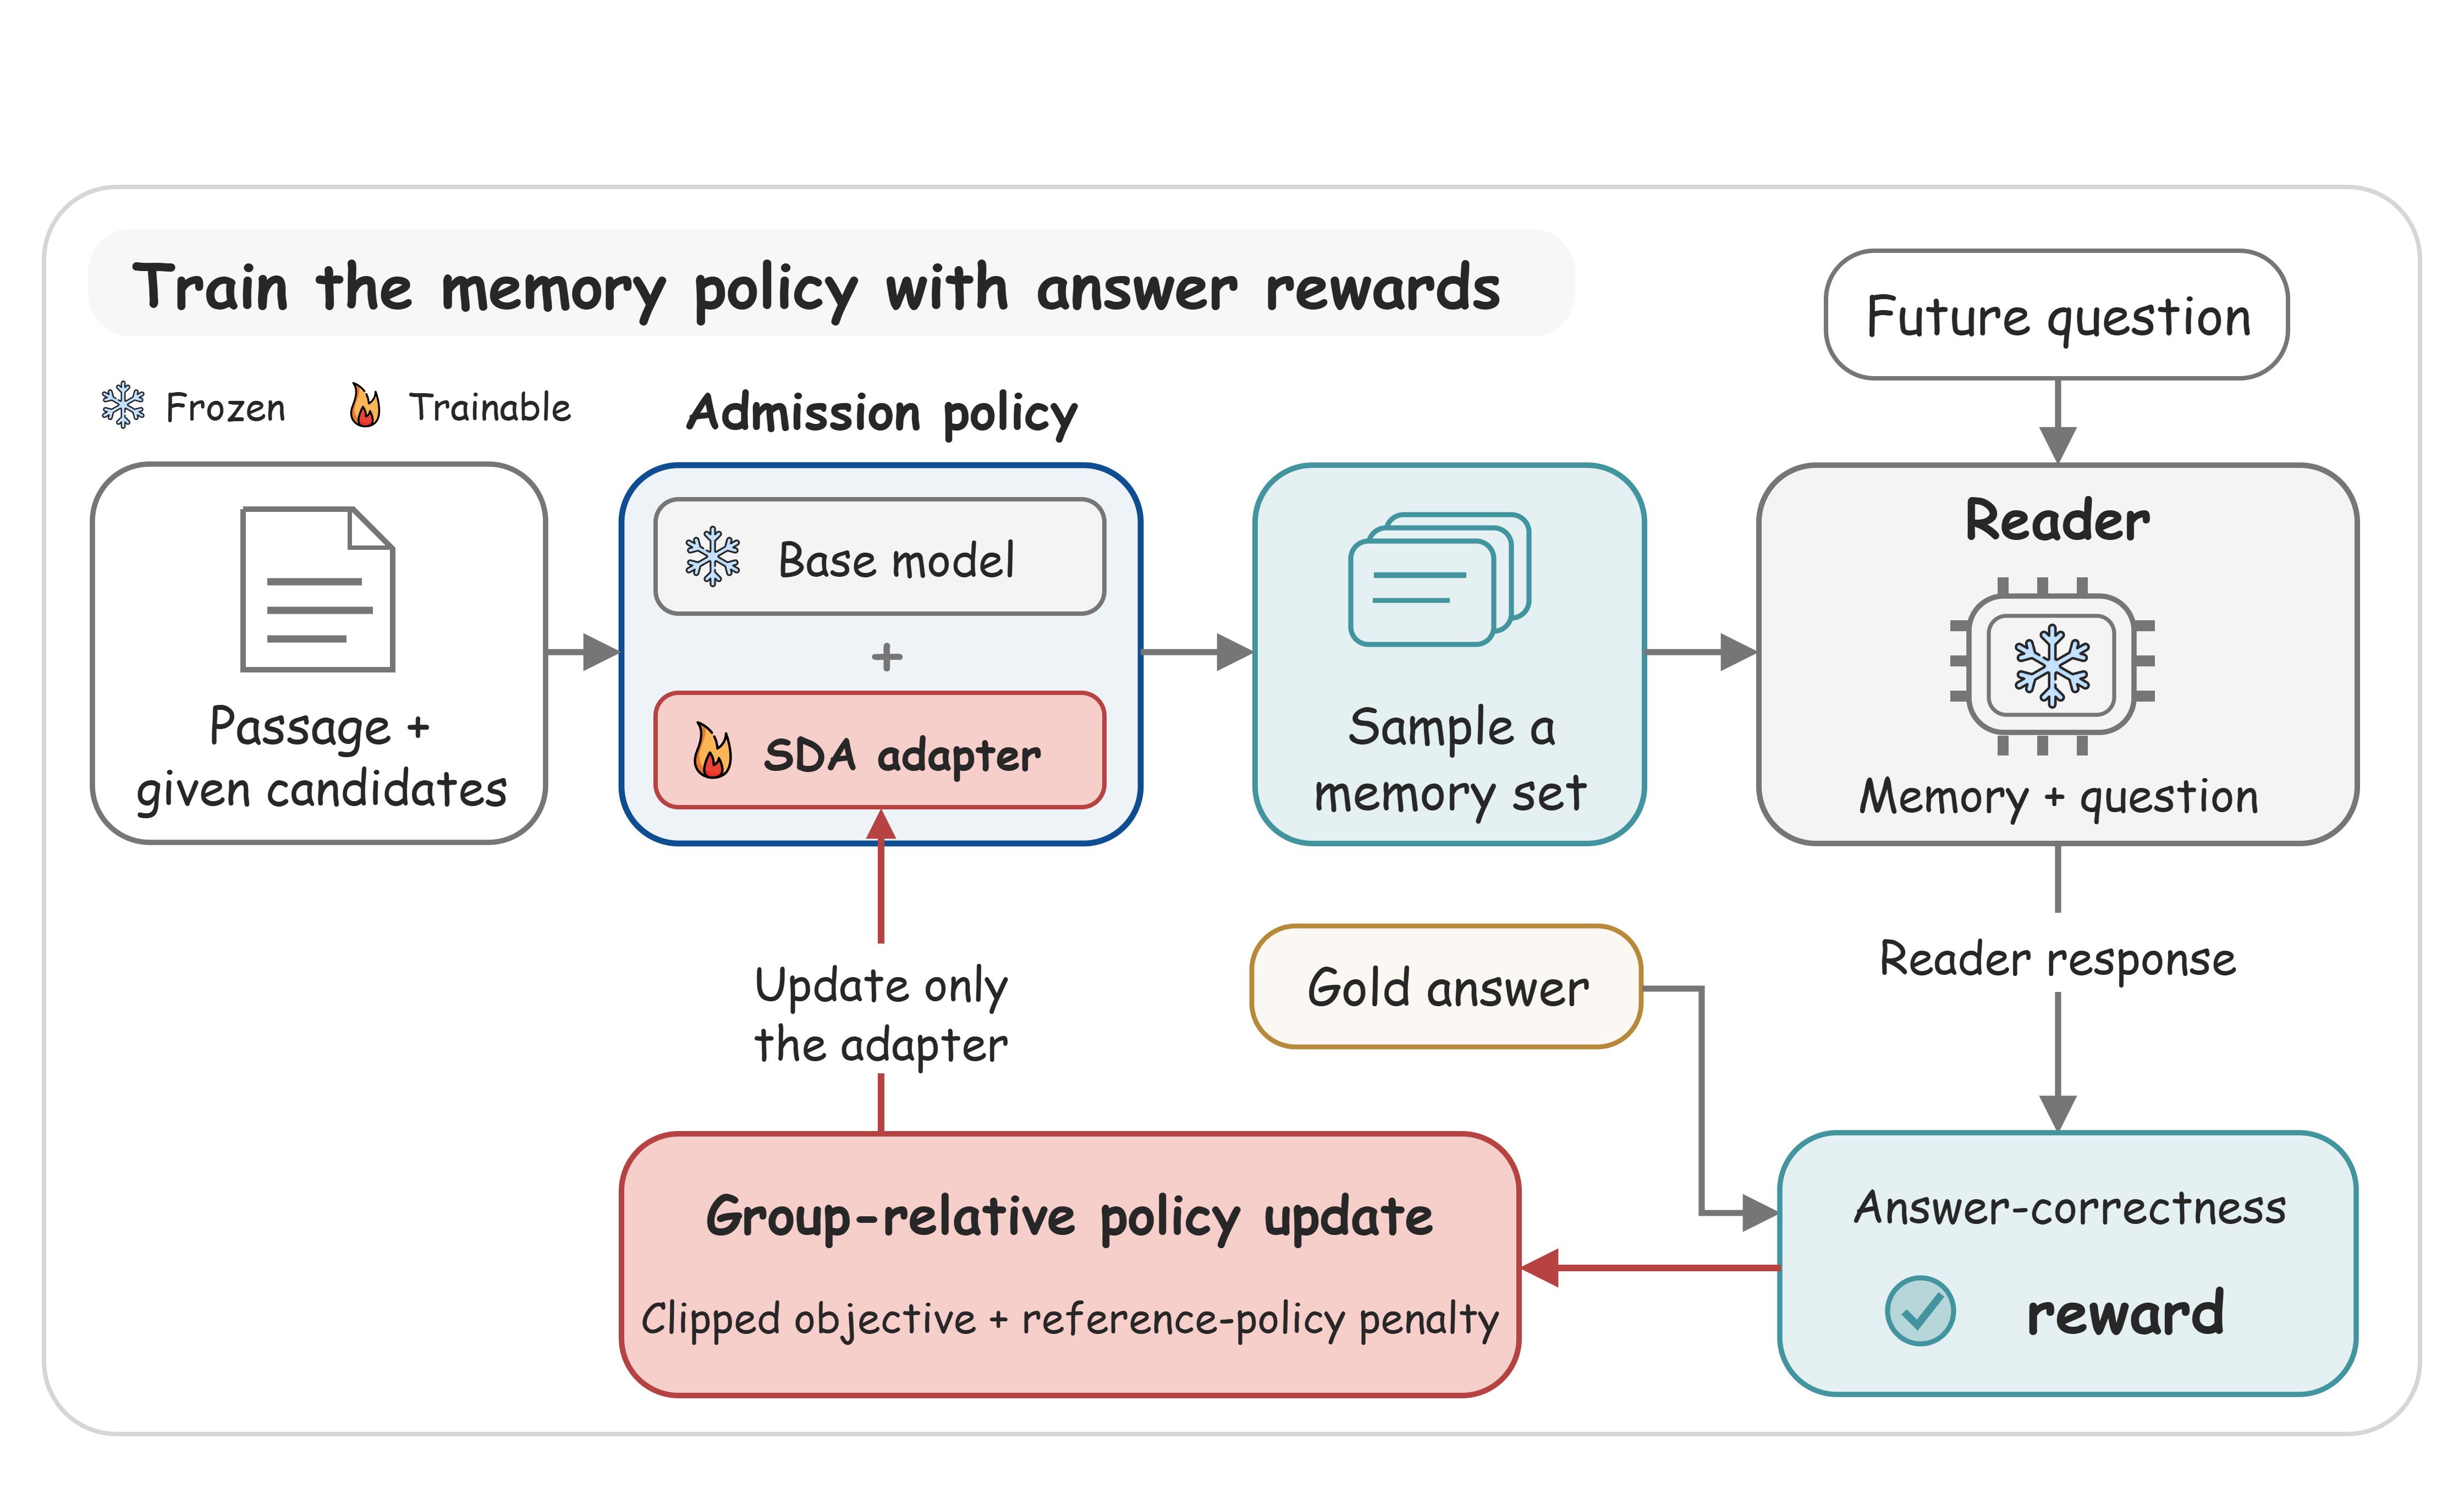
\includegraphics[width=\columnwidth,trim=0 20bp 0 56bp,clip]{figures/fig5.png}
\caption{Accuracy-reward training replaces distillation or refines the adapter after SDA. Group-relative policy updates train only the adapter using the frozen reader's answer correctness. The future question enters the reward computation.}
\label{fig:appreward}
\end{figure}

Accuracy reward uses the same training episodes and adapter shape with a matched step budget. Admitted sets are sampled from admission scores, and the frozen reader answers from the selected memory (Figure~\ref{fig:appreward}). Answer correctness supplies the reward. Within each rollout group, reward differences are normalized into advantages; updates use a clipped group-relative policy objective and a penalty for departure from the reference policy \citep{shao2024deepseekmath}. Refinement applies these updates after SDA training. SDA's labels come from the frozen model without a future question, answer or reward; reward training requires the future question and gold answer to compute rewards. On the original pool (Qwen3-8B, $k=2$; Table~\ref{tab:sdaablation}), accuracy reward replacing distillation reaches 46.4\%, 3.7 points below SDA; with question supervision, refinement builds on SDA to reach 52.9\%, 2.8 points above it.

\FloatBarrier
\section{Prompts}
\label{app:promptlist}

The prompts below give the instructions for the evaluated models, the
generator and the judge. Prompt~\ref{prompt:author} is the prose
transcription described in App.~\ref{app:authorprompt}; instructions for
unstated distractors and the judge's output format are described in
App.~\ref{app:pools} and App.~\ref{app:judge}, respectively.
Italic phrases stand for the supplied passage, candidate, memory list or
question.

\begin{sdabox}[prompt]{Episode generation}[prompt:author]
Design a batch of diverse test episodes about silent bridge reasoning
for a memory experiment. Each episode has a passage of four to eight
sentences about a named person; invent a distinctive first name,
different in every episode, and vary the domain widely. A question
asked later, out of context, refers to the episode only through the
person's name and requires an unstated bridge fact inferable from the
passage, followed by common general knowledge. Supply a short correct
answer of one to three words and five to seven candidate concepts,
each a common lowercase word with a utility category and a short reason.

Exactly one candidate is the useful bridge concept, and its word must
be absent from the passage. The question must share no passage content
word except the person's name: someone who never read the passage
must be unable to answer it. For a passage about Elena wandering the
Plaza Mayor, ask what language Elena should have brushed up on for her
trip, without naming the plaza in the question. The answer must differ
from every candidate and be absent from the passage; combining the
bridge with general knowledge yields the answer. For example, the
Plaza Mayor cues \emph{madrid}, which supports \emph{spanish}. A reader
remembering only the bridge plus the question must be able to answer.

Include two or three vivid, emotional or surprising distractors that
occur literally in the passage but are useless for the question, and
one or two neutral concepts that occur in the passage. Every candidate
must be a single common English lowercase word. Do not reuse concepts
or person names across episodes.
\end{sdabox}

\begin{sdabox}[prompt]{Importance prompt, shared by SDA and the report}[prompt:admission]
\emph{Passage}

Based only on the passage above, is the concept ``\emph{candidate
concept}'' one of the most important things to remember in order to
answer possible future questions? Answer with a single word: yes or no.
\end{sdabox}

\begin{sdabox}[prompt]{1--10 importance rating}[prompt:rating]
\emph{Passage}

On a scale of 1 to 10, where 1 is purely mundane and 10 is extremely
important, rate how important it is to remember the concept
``\emph{candidate concept}'' in order to answer possible future questions
about this passage. Answer with a single number.
\end{sdabox}

\begin{sdabox}[prompt]{ConsistencyGate, sampled form}[prompt:cgsample]
You are a fact-checking assistant. Given a source context and a
candidate fact, rate how strongly the fact is supported by the context.

Source context: \emph{passage}\\
Candidate fact: \emph{candidate concept}\\
Question: How strongly is this candidate fact supported by the source
context above? Do not use outside knowledge.

0.0 = completely unsupported or directly contradicted by the context\\
0.5 = partially supported or ambiguous\\
1.0 = fully and directly supported by the context

Output only a single decimal number between 0.0 and 1.0.
\end{sdabox}

\begin{sdabox}[prompt]{ConsistencyGate, single-pass form}[prompt:cgyesno]
You are a fact-checking assistant. Given a source context and a
candidate fact, decide whether the fact is supported by the context.

Source context: \emph{passage}\\
Candidate fact: \emph{candidate concept}\\
Question: Is this candidate fact supported by the source context above?
Do not use outside knowledge.

Answer with a single word: yes or no.
\end{sdabox}

\begin{sdabox}[prompt]{A-MAC utility}[prompt:amac]
\emph{passage}

Consider storing the concept ``\emph{candidate concept}'' in long-term
memory. Is it actionable, does it support likely follow-up questions, or
does it capture a persistent constraint or preference?

Answer with a single word: yes or no.
\end{sdabox}

\begin{sdabox}[prompt]{Frozen reader}[prompt:reader]
Earlier you read a passage. The only things you remember from it are:
\emph{stored concepts separated by commas}.\\
Using only what you remember, answer concisely.\\
Question: \emph{future question}\\
Answer:
\end{sdabox}

\begin{sdabox}[prompt]{Blind semantic judge}[prompt:grading]
Grade short answers to memory questions. For each item decide whether
ANSWER gives GOLD as its answer.\\
Labels:\\
``correct'': the answer commits to GOLD or an exact equivalent (synonym,
inflection, fuller name) as its single answer. Extra explanation is fine.\\
``hedged'': it offers two or more alternative answers (e.g.\ ``X or Y''),
or states the answer cannot be determined, even if GOLD is mentioned.\\
``incorrect'': anything else, including a different answer.
\end{sdabox}
